% !TeX root = ../main.tex

\chapter{电激发瞬态吸收光谱仪的原理及搭建工作(包含LabVIEW操控系统)}
\section{引言}
泵浦-探测技术是一种利用短激光脉冲测量超快现象的技术,在物理学、化学、材料科学等领域有着广泛的应用。该技术最早由Toepler\cite{toepler1867optische}提出,其基本工作原理是利用飞秒脉冲激光器作为光源,通过分束镜将激光分为两束光,可以通过光学延时线调节两束光之间的时间延迟,通常我们把其中能量较高、时间较前的作为泵浦光,能量较低、时间延后的作为探测光。泵浦光先照射到样品上,激发样品到达激发态,具有一定时间延迟的探测光随后到达,探测样品受到激发后随时间的演化。利用光电探测器检测光经过样品后的信号变化,并可通过锁相放大器等设备进一步提高信噪比,最终可以得到较好的样品时间分辨信息。目前该技术已被广泛应用于物理、化学、材料和生物等领域,特别是用于研究物质的瞬态响应和动力学行为。
\section{电激发瞬态吸收光谱仪}
\subsection{瞬态吸收光谱}
瞬态吸收光谱(Transient Absorption Spectroscopy, TAS)是以一种基于泵浦-探测技术的超快时间分辨的光谱探测技术,用于测探材料激发后的瞬态行为,特别是激发态载流子布居的动力学过程。脉冲激发的瞬态吸收光谱可以排除样品在脉冲电激发下发光引起的电致发光信号和光导效应引起的额外电流的光信号,实现对电注入的单电子、单空穴和电子-空穴对的动力学。此外,瞬态吸收光谱技术最大的一个优点是可以探测不发光样品的激发态动力学,这非常有利于我们去对比好与坏的器件的差异,以及可以通过对照实验减去如量子点层或者某传输层来确定对应层级信号。
\begin{figure}[ht]
	\centering
	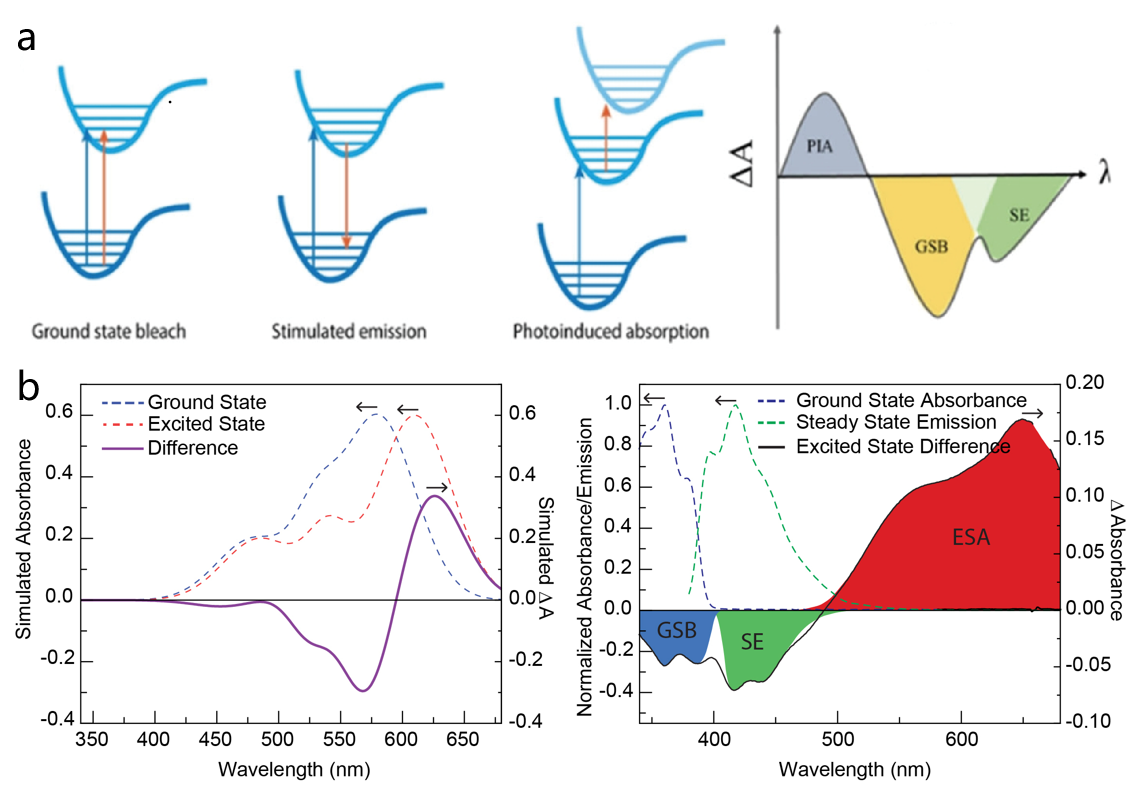
\includegraphics[width=\textwidth]{TAS.png}
	\caption{瞬态吸收光谱信号$\Delta A$。图a,信号来源示意图\cite{srivastava2023advanced}。图b,代表性TA光谱模拟\cite{jove65519}。}
	\label{fig:TAS}
\end{figure}
瞬态吸收光谱的公式表示为:
\begin{equation}
	\Delta A=\lg I_{pump}-\lg I_{unpump}.
	\label{eq:1}
\end{equation}
其中$I_{pump}$和$I_{unpump}$分别为有无泵浦光时的探测光强度。如图\ref{fig:TAS}所示,$\Delta A$的贡献主要来源于激发态吸收(Excited State Absorption, ESA)、光诱导吸收(Photoinduced Absorption,PIA)、基态漂白(Ground State bleaching, GSB)和受激辐射(Stimulated Emission,SE)这四部分。具体地:
\begin{enumerate}
	\item 激发态吸收:样品受激发后,激发态粒子吸收探测光能量被进一步激发跃迁到更高能级上,对$\Delta A$表现为正贡献。
	\item 光诱导吸收:光激发引起样品发生光化学反应,生成的中间态吸收探测光,对$\Delta A$表现为正贡献。
	\item 基态漂白:样品受激发导致基态粒子数减少,直接导致对探测光的吸收下降,对$\Delta A$表现为负贡献。
	\item 受激辐射:激发态粒子在同频光子作用下弛豫到基态并辐射光子,对$\Delta A$表现为负贡献。
\end{enumerate}

\subsection{电激发瞬态吸收光谱仪}
传统的TAS光激发基于吸光度的变化判断样品中处于激发态和基态的载流子布居变化,仅能得到样品中载流子弛豫的动力学行为,可适用于QDs薄膜等简单结构,但对于QD-LED器件,多层结构导致的载流子注入行为无法探测,特别是由于电激发导致的载流子注入过程中的激发态跃迁,因此光激发瞬态吸收光谱仪此时将不再适用。Fan课题组通过使用电脉冲信号替代传统的飞秒激光器给出的光脉冲信号,成功实现了基于电激发的瞬态吸收光谱技术(Electrically Excited Transient Absorption Spectroscopy, EETA)\cite{li2024transient,1025004826.nh},基于此技术,成功探测到了QD-LED器件稳态的载流子平衡浓度以及动力学和电场分布等信息。
\begin{figure}[ht]
	\centering
	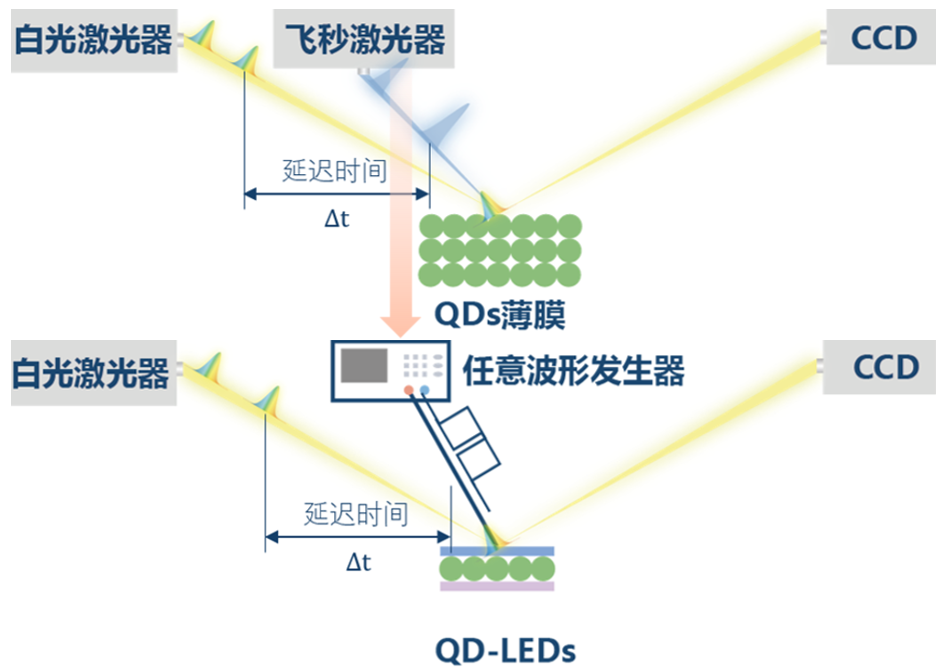
\includegraphics[width=.8\textwidth]{eeta1.png}
	\caption{EETA(下)与传统TAS(上)对比示意图\cite{bian2024efficient}。}
	\label{fig:eeta1}
\end{figure}

电激发瞬态吸收光谱$\Delta A$的表达式为:
\begin{equation}
	\Delta A=\lg \dfrac{I^{probe}_{pump}}{I^{ref}_{pump}}-\lg \dfrac{I^{probe}_{unpump}}{I^{ref}_{unump}}.
	\label{eq:2}
\end{equation}
其中其中$I^{probe}_{pump}$和$I^{probe}_{unpump}$分别是有无电激发的探测光强度,$I^{ref}_{pump}$和$I^{ref}_{unpump}$分别是有无电激发的参考光强度。文献\cite{1025004826.nh}中给出了电激发瞬态吸收光谱$\Delta A$的理论模型表达式:
\begin{equation}
	\begin{aligned}
		\Delta A=&-\dfrac{2\sigma N_en_{QD}l_{QD}}{2.303}+\dfrac{2(1-N_e)n_{QD}l_{QD}}{2.303}\left(E\dfrac{\partial \nu}{\partial E}+E^2\dfrac{\partial^2 \nu}{\partial E^2}\right)\dfrac{\partial \sigma}{\partial \nu}\\
		&+\dfrac{2E^2(1-N_e)n_{QD}l_{QD}}{2.303}\left(\dfrac{\partial \nu}{\partial E}\right)^2\dfrac{\partial^2 \sigma}{\partial \nu^2}.
		\label{eq:3}
	\end{aligned}
\end{equation}
\begin{figure}[ht]
	\centering
	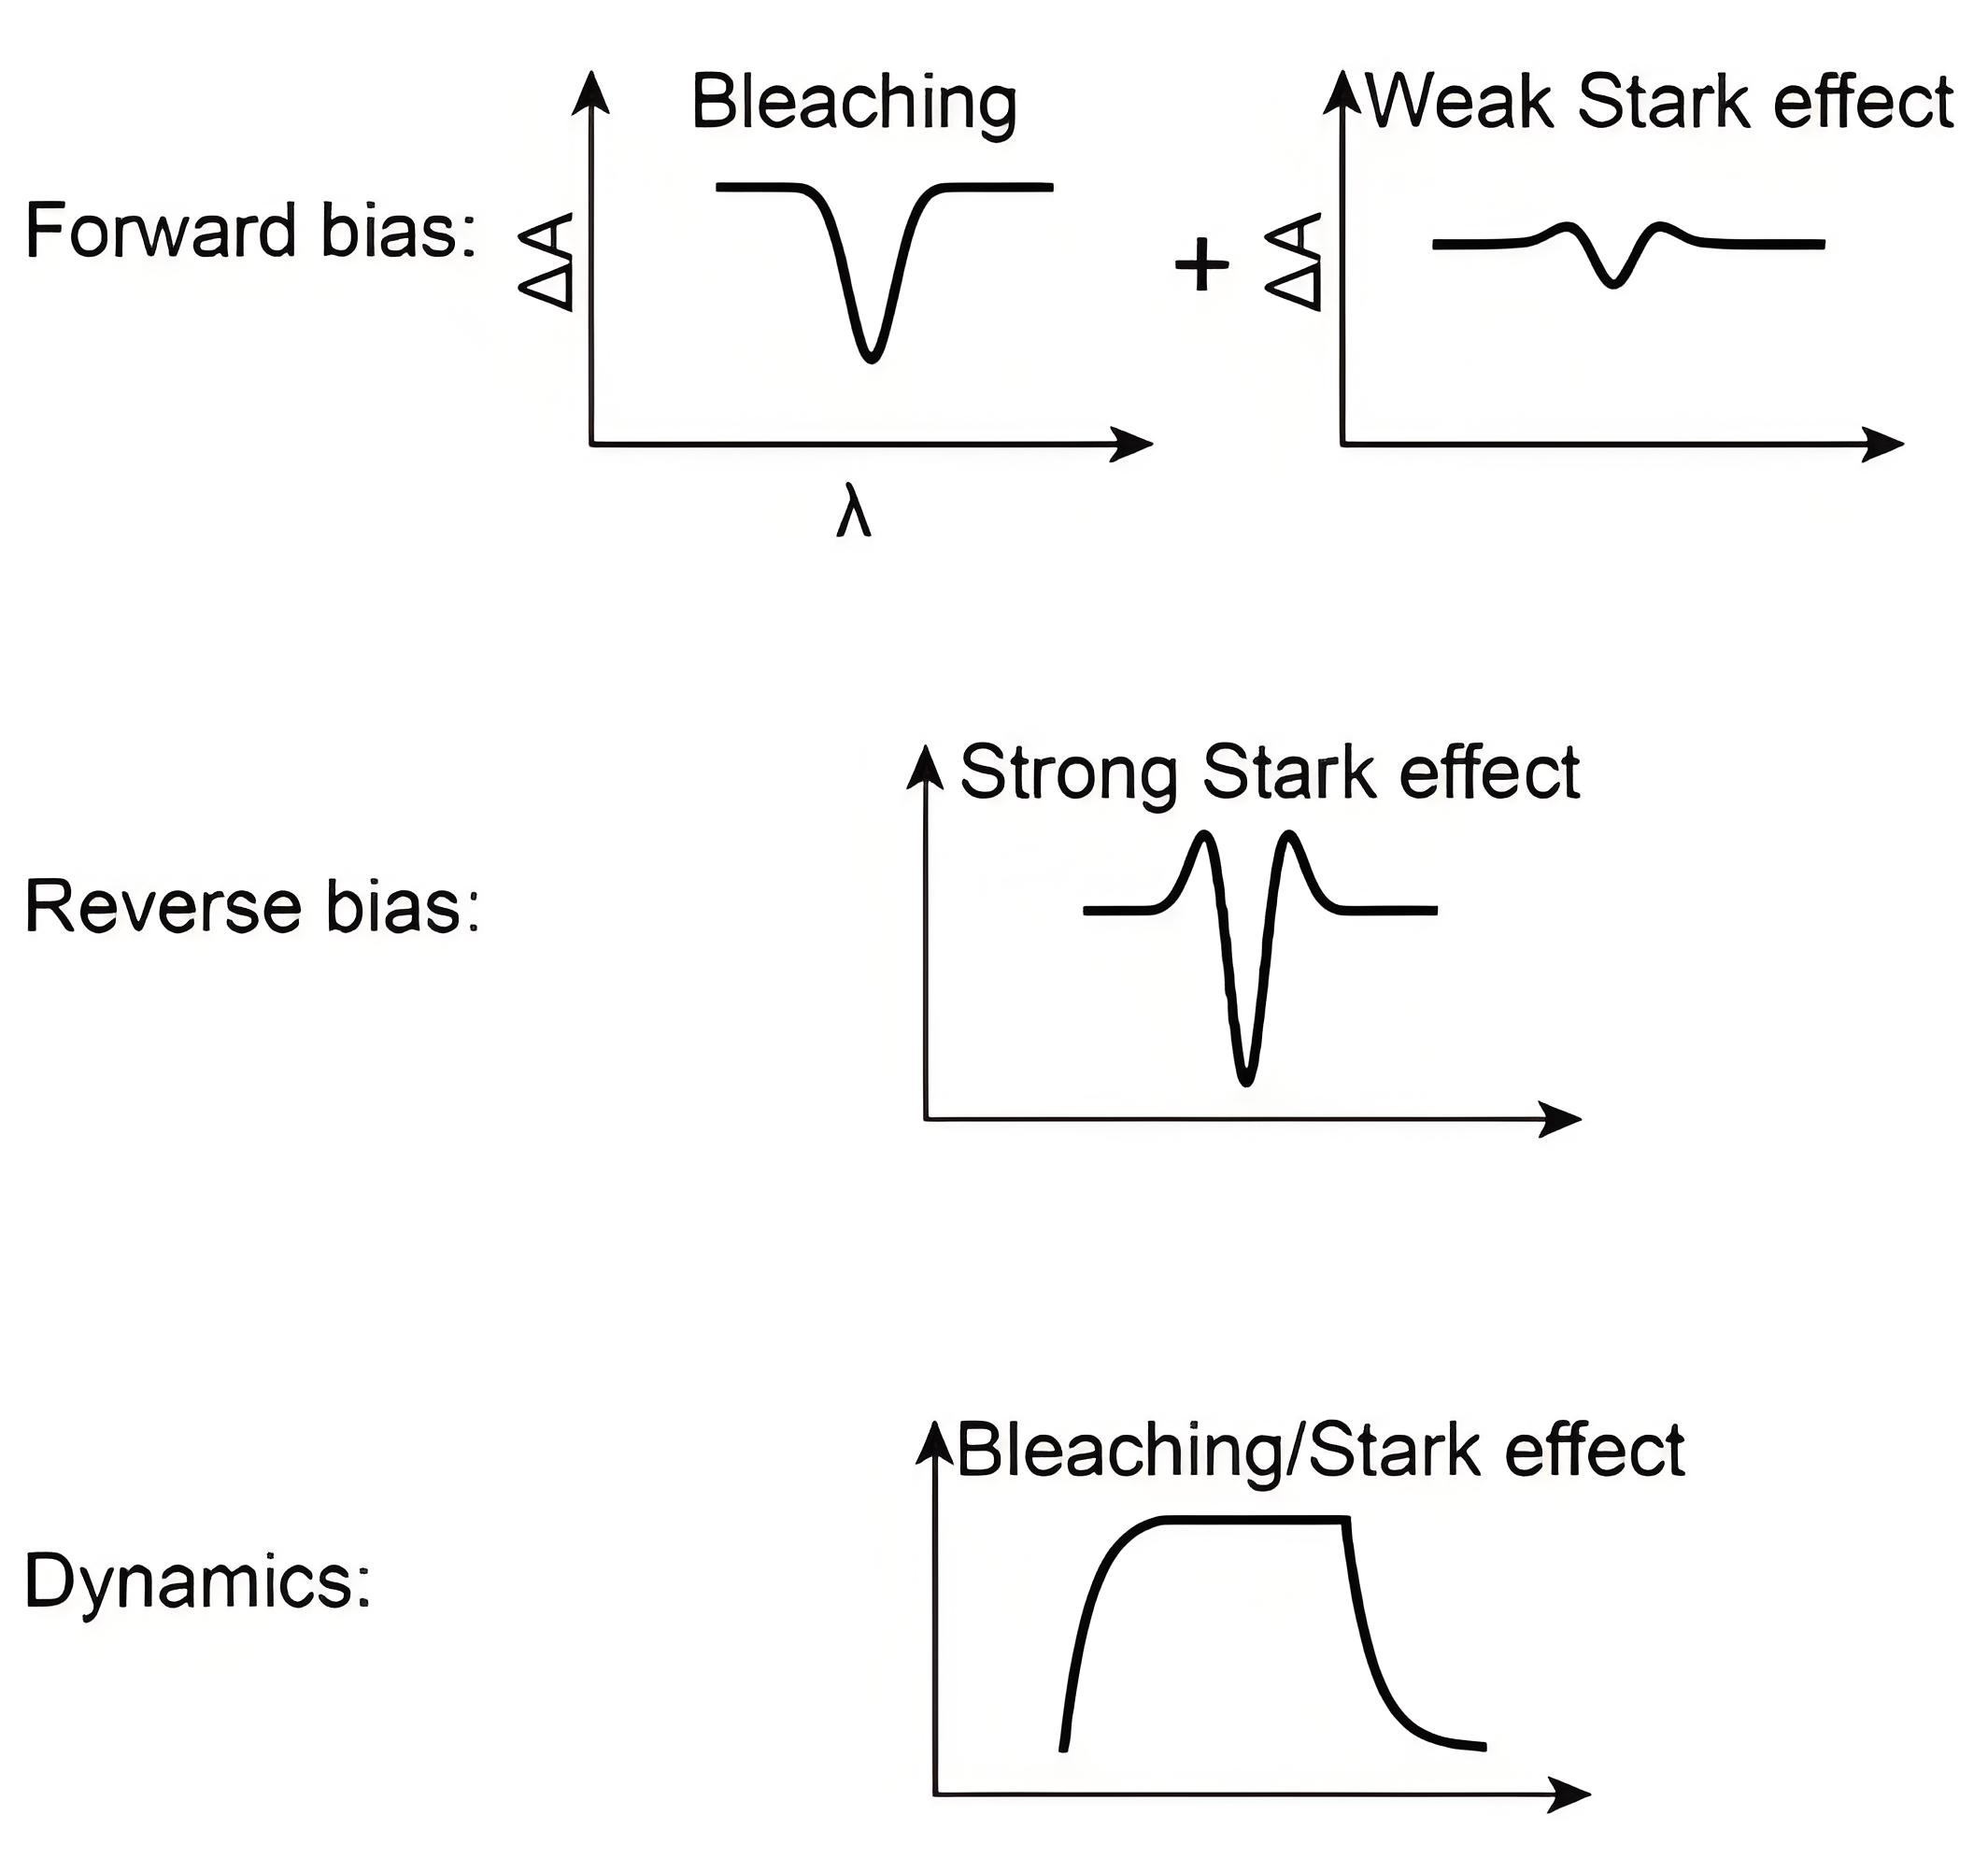
\includegraphics[width=.6\textwidth]{1.jpeg}
	\caption{斯塔克和漂白信号示意图\cite{acs.nanolett.4c03024}。}
	\label{fig:1}
\end{figure}
其中$\sigma$是无外电场时的吸收截面,$E$是外电场强度,$\nu$是波数,$n_{QD}$和$l_{QD}$分别是无外电场时的量子点层的密度和厚度,$N_e$是外电场下量子点密度。表达式\ref{eq:3}中第一项为漂白信号(Bleaching),反映量子点层平均电子数和相对电场强度,后两项分别为一阶和二阶斯塔克效应(Stark Effect),反映的是量子点的固定偶极和诱导偶极。图\ref{fig:1}展示了在正向偏置条件下,光谱信号包含微弱的斯塔克效应和较强的漂白信号;而在反向偏置条件下,可以获得更强的斯塔克效应信号。通过调节泵浦-探测延迟时间,可以获取漂白和斯塔克效应的动力学信息。


通常,对于QQ-LED器件,如图\ref{fig:rolloff}展示的多层结构,各个功能层对应的吸收峰往往是不相重的,因此,我们往往选取白光作为探测光,利用其极宽的光谱范围(通常可以覆盖300-1000nm以上的紫外-可见-红外全光谱)可将各个峰位信号较为容易的定位到各个功能层,由此来确定各个功能层的载流注入动力学和平均浓度以及电场信息,这也是电激发瞬态吸收光谱的天然优势所在。
\begin{figure}[ht]
	\centering
	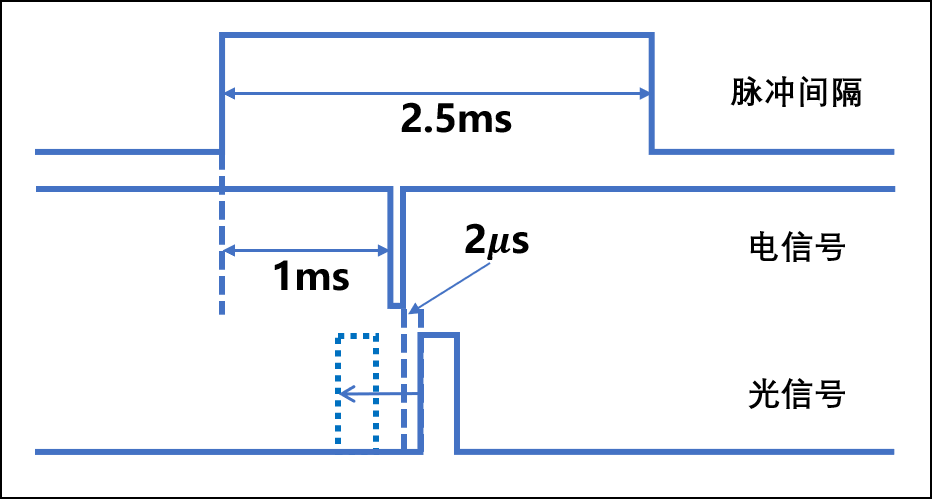
\includegraphics[width=.8\textwidth]{AWG.png}
	\caption{AWG触发信号初始相位示意图。}
	\label{fig:AWG}
\end{figure}
\subsubsection{EETA搭建工作}
本工作搭建了一台紫外波段拓展的电激发瞬态吸收光谱仪,示意图如图\ref{fig:EETA}所示。其中探测光采用白光光源,其光谱范围约为195nm-1100nm(实际最高只能达到800nm),通过任意波形发生器(Arbitrary Waveform Generator,AWG)提供200Hz的晶体管-晶体管逻辑电平(Transistor Transistor Logic, TTL)触发脉冲信号。因为我们需要CCD检测有无电激发的探测光强度,因此在这里我们给两个CCD提供相同的400Hz的触发信号,同时给LED样品提供400Hz的电脉冲信号,三者通过AWG实现初始零点同步。这里电脉冲信号的宽度设置为10$\mu s$,远小于400Hz(等价于2.5ms)的脉冲间隔,我们知道半导体中电荷自然耗散的时间在$\mu s$级别,因此可以确保各功能层的载流子注入达到稳态。图\ref{fig:AWG}展示了这三个信号初始相位的差异,其中初始电信号和光信号设置在每个间隔中间位置,以确保能完整的检测整个过程,光信号约滞后于电信号的目的是在移动光脉冲信号时能检测完整的下降沿。

\begin{figure}[ht]
	\centering
	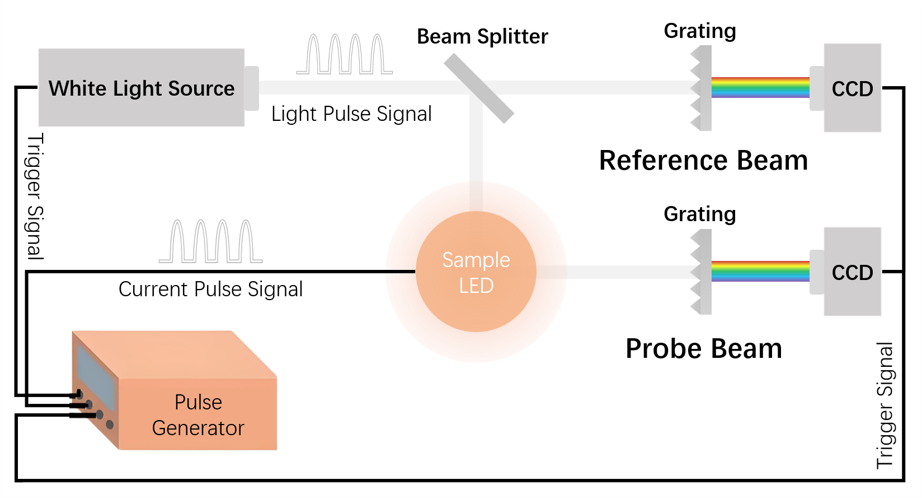
\includegraphics[width=\textwidth]{EETA.png}
	\caption{电激发瞬态吸收光谱仪结构示意图。}
	\label{fig:EETA}
\end{figure}

白色光源给出的光脉冲信号经过分束器分为两束光,其中一束光作为参考光直接通过光栅被CCD检测,另一束光作为探测光探测LED器件,反射光通过光栅被另一个CCD检测。实验中发现直接给CCD提供一系列脉冲信号可能会因为延迟等因素导致CCD获取到不完整或是缺失的触发信号,这会导致可能某些时刻因为CCD没有触发而导致数据缺失,因为我们计算电激发瞬态吸收光谱$\Delta A$需要相邻的有电激发和无电激发时的探测光强度,而我们没有办法去检测数据是否是有电激发的,在整体法处理数据时就可能会产生无电激发信号减有电激发信号/无电激发信号减无电激发信号/有电激发信号减有电激发信号的情况,如此我们会得到错误的光谱信息,第一种情况还可以通过翻转光谱数据修补,但后二者基本无法补救。为解决该问题,我们在原先的基础上增加了一台国仪量子ASG8100数字延时脉冲发生器作为中介,AWG给出的触发信号不直接给到CCD而是通过ASG8100的IN接口接收进而输出一个一个完整的触发信号给到CCD,从结果上看,成功解决了上述问题。但本仪器仍存在一些不足,主要在于光源的高弛豫时间,只能达到300-400ns左右的分辨率,而载流子弛豫时间一般在皮秒到纳秒级别,因此只能探测稳态时载流子的信息而无法探测载流子动力学过程的信息。下图\ref{fig:ETA}即为我们本文搭建的紫外波段拓展的电激发瞬态吸收光谱仪。
\begin{figure}[ht]
	\centering
	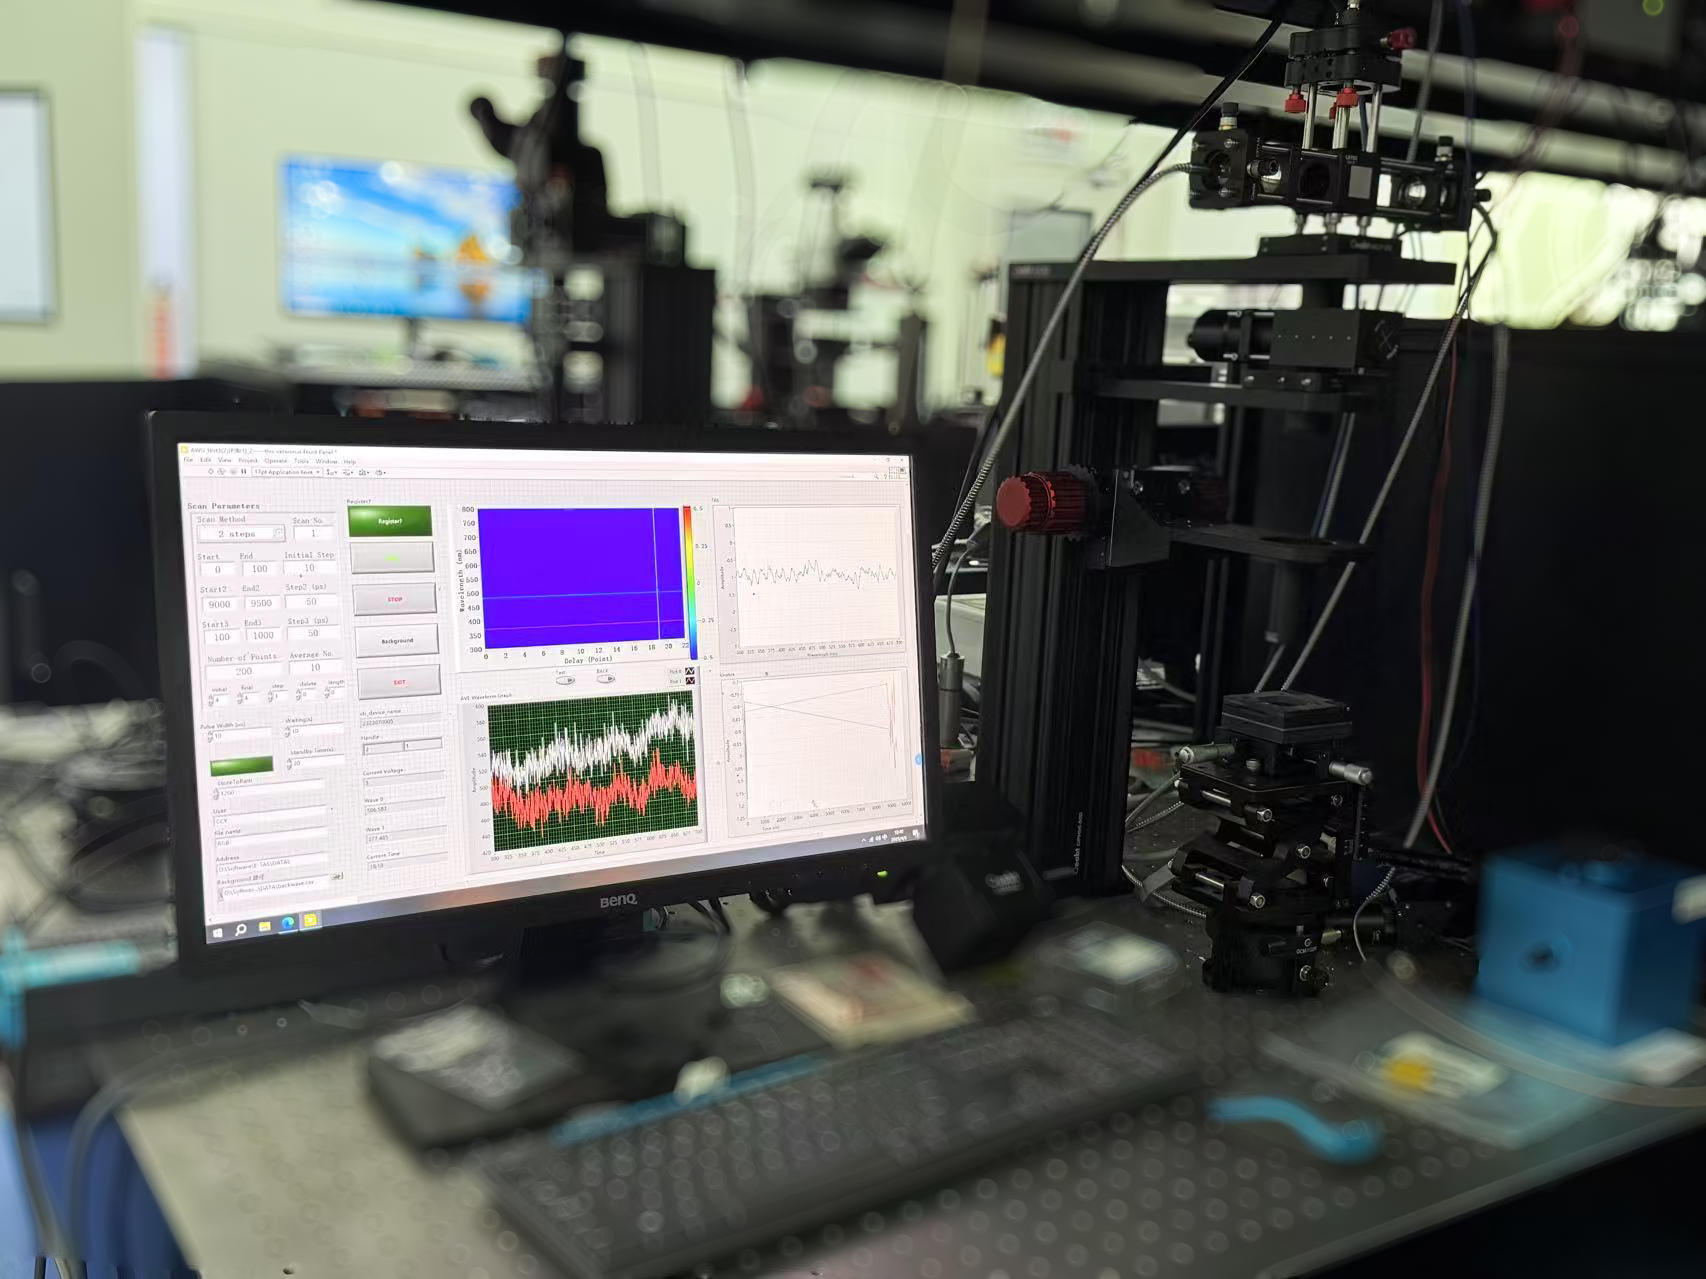
\includegraphics[width=.8\textwidth]{ETA.png}
	\caption{电激发瞬态吸收光谱仪。}
	\label{fig:ETA}
\end{figure}
\subsubsection{LabVIEW操控系统}
我们利用LabVIEW实现了对上述完整测量流程的一体化操控。由于具体代码较为复杂且流程较长,这里仅仅展示前面板,如图\ref{fig:qmb}所示,其中(1)是扫描参数,可以设置一步法、两步法、三步法以及指数法和线性法,包含平均扫描次数以及电压始末设置;(2)是每次CCD最长测量时间,一旦超出将自动退出程序,目的是为了防止发生错误时CCD超时;(3)是待机时间,开启后当主程序达到待机时长后自动退出程序;(4)是CCD每次测量存入内存的数据组数目;(5)是储存和读取的文件路径设置;(6)是主要控件;(7)是运行时间;(8)是电激发瞬态吸收谱(EETA),可移动两横线来得到两波长下的动力学图像,也可移动竖线来管擦对应Delay下的TAS谱;(9)的Plot0和Plot1分别对应探测光和参考光,可以实时显示测量时对应的光谱信息;(10)(11)分别是TAS谱和动力学图像,其中TAS谱展示的是EETA中的黄色竖线位置的数据,而动力学图像展示的是EETA中红色和蓝色横线位置的数据;(12)使程序以当前参数持续运行,并可利用(5)中的控件控制,主要便于调试光路时观察(9);(13)用于自动测量当前参数下的无光时的背底数据,并放入固定数据文件中,正常测量时将自动减去该背底。
\begin{figure}[ht]
	\centering
	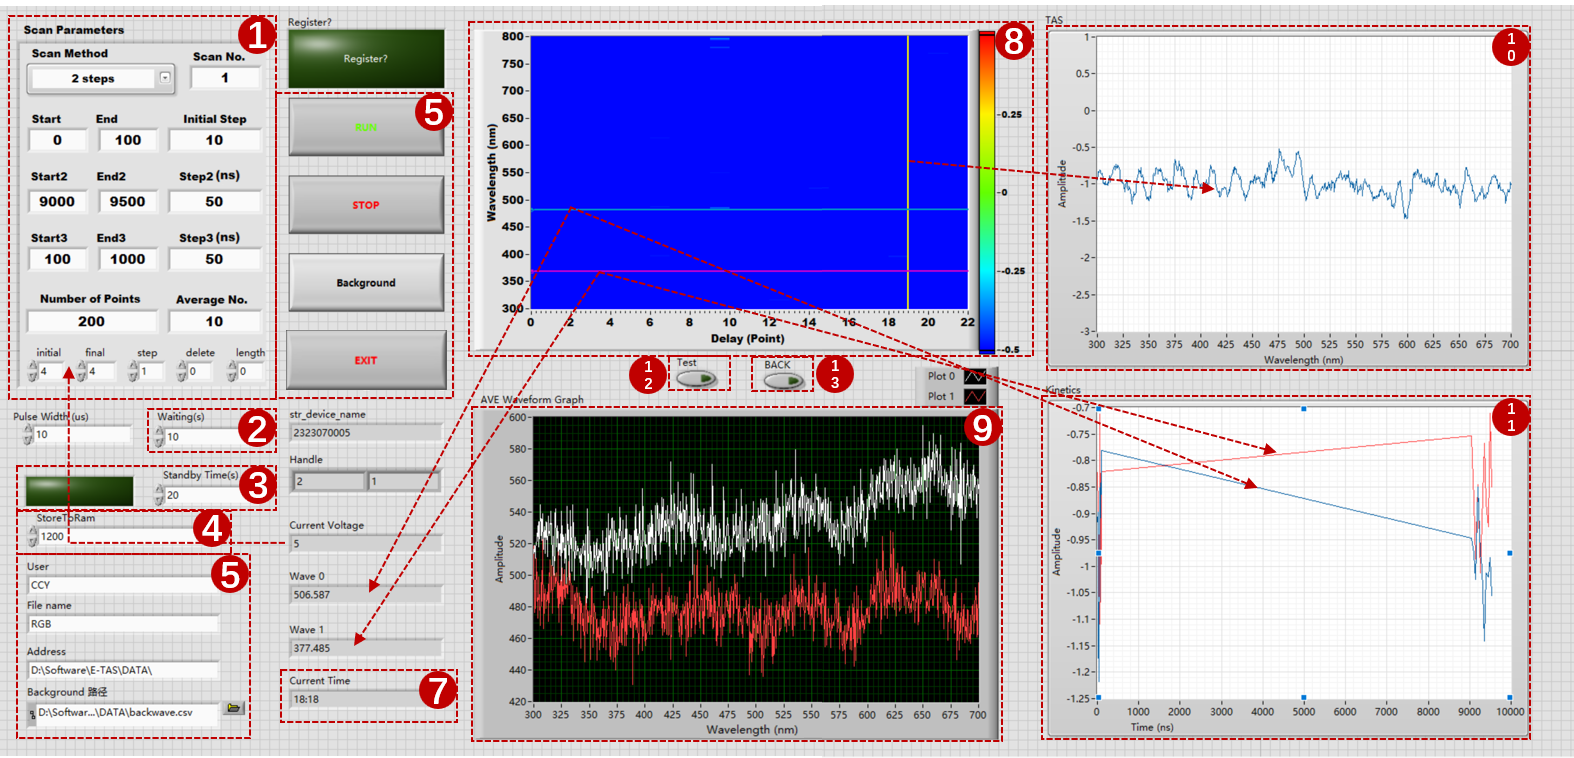
\includegraphics[width=\textwidth]{前面板.png}
	\caption{LabVIEW操控系统前面板。}
	\label{fig:qmb}
\end{figure}
\subsection{电激发瞬态吸收光谱的数据分析方法}\label{2.3}
通过图\ref{fig:1}我们知道,正向偏置时,光谱信号主要由Bleaching信号和弱Stark信号贡献,Bleaching信号反映的是各功能层基态和激发态粒子布居的变化行为,而Stark信号反映的是电场的信息;而在反向偏置下,光谱信号主要是由强Stark信号贡献。下面我们将详细展开说明下这两种信号。
\subsubsection{Bleaching信号}
Bleaching信号(基态漂白,GSB),是由于泵浦光谱脉冲将分子从基态激发到激发态而导致的基态分子数目减少,在TAS中表现为探测光在基态吸收峰减小,因而表现出TAS谱中表现出一个“凹陷”,因此,Bleaching信号地能量位置往往与基态吸收峰一致,其形状和宽度可以反映激发态密度变化和局域场效应。此外,Bleaching信号地衰减行为通常与激发态粒子辐射或非辐射复合、载流子弛豫以及基态恢复过程有关,可以从中提取出激发态寿命、载流子扩散以及其他非平衡动力学参数,这可以帮助我们研究材料的超快动力学。
\subsubsection{Stark信号}
Stark效应是指由于外加电场导致的原子或分子的谱线移动和分裂的现象,该效应本质上是改变了电子能级和跃迁偶极矩。在光谱学中,Stark效应的表现包括线性Stark效应(正比于电场)和二次Stark效应(与电场平方成正比),通常后者更为常见。在TAS谱中,Stark效应影响能级移动、偶极矩变化和点和动力学的调制,将会显著改变谱线形状和动力学行为。具体地,我们可以总结为以下几点:
\paragraph{谱线位移}
\subparagraph{一阶Stark效应}
对于具有非零永久偶极矩的分子,在电场作用下,基态和激发态的能量会发生线性移动,其能量改变量$\Delta E$与电场强度$E$成正比,并且与偶极矩$\mu$和电场方向的夹角有关$(\Delta \symbf{E}=-\symbf{μ}\cdot\symbf{E})$。由于基态和激发态的偶极矩通常不同,因此电子跃迁的能量差也会发生改变,导致瞬态吸收光谱的峰位发生移动。
\subparagraph{二阶Stark效应}
所有分子都具有极化率。电场会诱导分子产生额外的偶极矩,并与电场相互作用,导致能级发生二次移动,此时其能量改变量$\Delta E$与电场强度$E$的平方成正比。基态和激发态的极化率差异会导致跃迁能量的改变,从而引起瞬态吸收光谱的峰位移动。二阶Stark效应通常比一阶Stark效应弱,但在具有对称性而导致永久偶极矩为零的分子中,二阶Stark效应成为主要的影响因素。
\paragraph{谱线展宽}
外加电场与不同取向的分子偶极矩的相互作用不同,导致不同分子的能级移动量不同,从而引起光谱的非均匀展宽。展宽的程度取决于偶极矩变化的大小和电场强度。对于多原子分子,电场还可能影响分子的振动模式,导致电子跃迁的振动结构发生变化,从而引起光谱的复杂展宽。
\paragraph{谱线强度变化}
电场可以改变跃迁的跃迁偶极矩强度,从而影响瞬态吸收光谱的强度。这种变化通常与电场诱导的分子波函数混合有关。外加电场还可能通过破坏分子的对称性使部分跃迁禁止被允许,导致在瞬态吸收光谱中出现新的峰或者原有峰的强度显著增加。
\paragraph{动力学影响}
Stark效应还会影响激发态的寿命、内转换、系间窜越等速率常数。这会间接地反映在瞬态吸收光谱的时间演化行为上。例如,电场可能改变激发态势能面的形状,从而影响反应路径和速率。
\begin{figure}[ht]
	\centering
	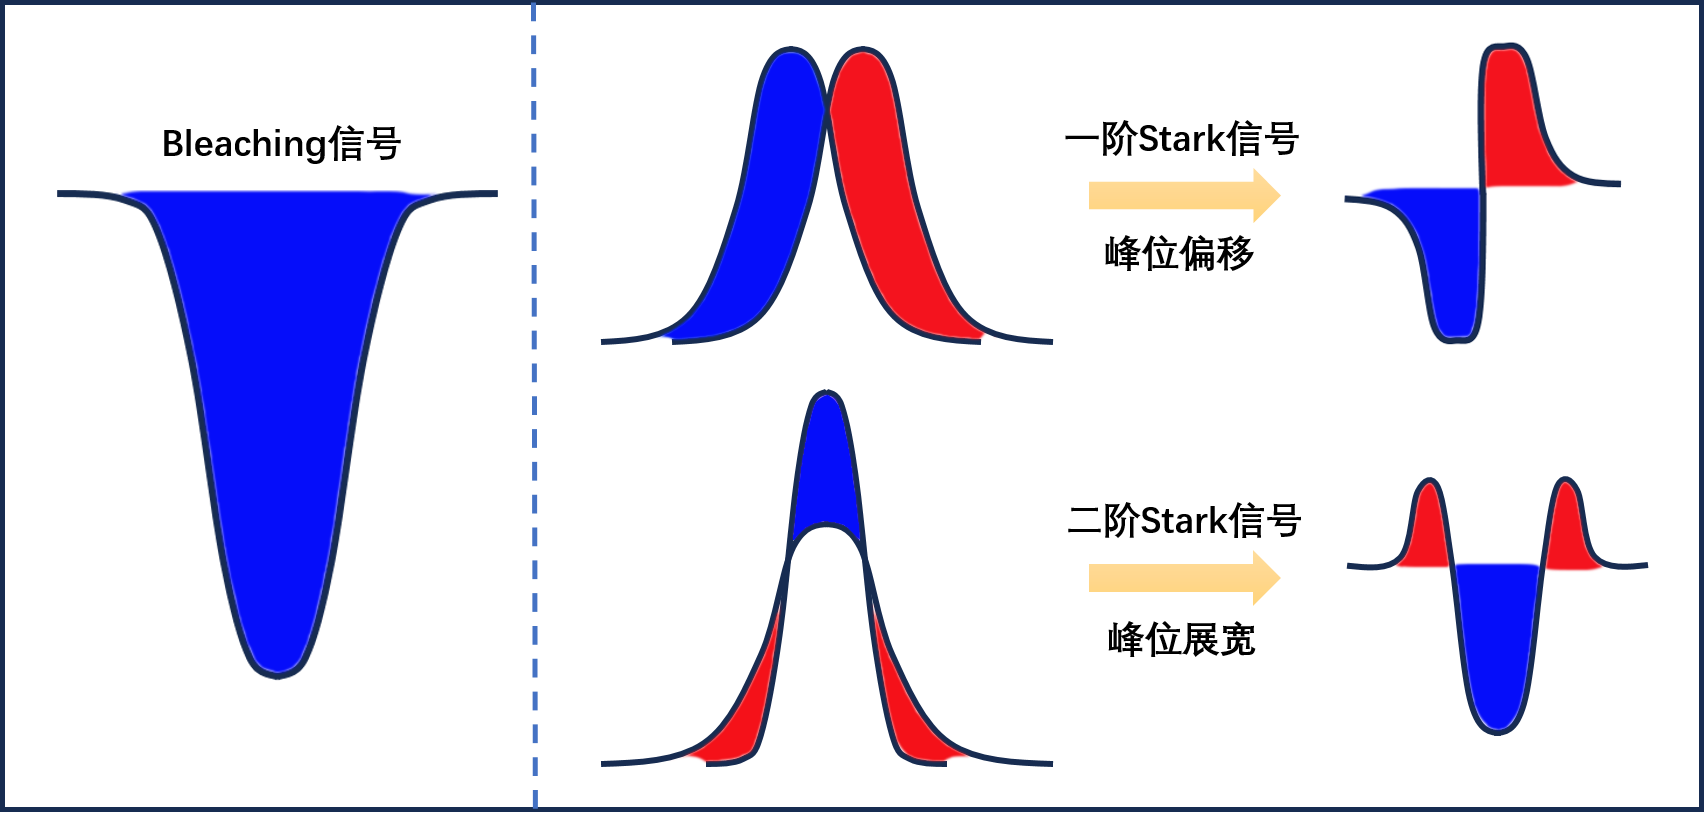
\includegraphics[width=\textwidth]{EETA信号.png}
	\caption{EETA中Bleaching信号和Stark信号的常见形态。}
	\label{fig:xh}
\end{figure}

通过表达式\ref{eq:2}我们知道,$\Delta$A主要由有无电激发时的探测光和参考光强度贡献,我们这里略作解释:可以认为有无电激发时的参考光强度对应于有无电激发时的探测光强度的归一化,因此,其本质上与TAS谱的表达式\ref{eq:1}是一致的,即表现有无电激发时候的探测光强度变化。如图\ref{fig:xh}展示了在电激发瞬态吸收光谱(EETA)中,Bleaching信号和Stark信号的常见形态。在光谱分析中,我们可以简单把Bleaching信号的强度归因于层中对应载流子的数目,二者为正相关。可以认为有电激发时器件中基态载流子吸收能量已经有一部分发生跃迁至激发态,相对于无电激发的情况,器件中基态载流子吸收光子而被激发的数目发生相对性的下降,因此体现了一个在对应吸收峰处的负值信号。而对于Stark信号而言,其强度大小则与电场强度有关,一定程度下表现出正相关,我们可以简单认为对某一功能层,当其相邻两侧功能层的电荷相反的载流子的相对数目增加时,产生的电场效应也增强,对应的Stark信号在一定程度上也会增强。在有电激发时,电场作用导致能级展宽或是偏移,体现在吸收峰上表现出峰位的移动或是由原先“高而窄”变为“低而宽”,因此有无电激发的探测光信号相减可以得到两种信号形态,对应着一阶Stark信号和二阶Stark信号。

在动力学研究中,即图\ref{fig:qmb}中(11)Kinetics图像,展示的是目标波长时$\Delta$A与Delay的关系,通常在零时刻其初值应该为零,但可能因为存在未删减初值导致非零初值。图\ref{fig:sl}给出了一个比较简单但典型的EETA谱示意图,包括TAS谱和动力学谱。我们可以看到,该动力学图像中存在一个下降沿、一个稳态和一个上升沿,其中下降沿主要由Bleaching信号引起,如果存在上升波动,则说明存在Stark信号,但通常正向偏置时,Stark影响为次要的,所以大体上呈现下降趋势,表明了该吸收峰所对功能层对应的载流子注入过程;稳态阶段,对应信号达到饱和,仅存在非理想导致的上下小波动;上升沿,测量结束,电压偏置回到零值,载流子发生弛豫,最后信号回到原点。我们还可以直接通过EETA谱观察载流子在各个功能层的行为,如图\ref{fig:sl}中的EETA谱,我们可以看到水平方向上存在两处偏离原点的负值,这对应较大的Bleaching信号,说明该波长对应功能层存在较多的载流子注入,而且也反映了一定的时间信息,比如说如果在某一Delay时存在相邻波长的$\Delta$A的负值发生整体在波长上的偏移,说明了在该时刻可能发生了原功能层载流子大量注入或泄露到新功能层的过程。

\begin{figure}[ht]
	\centering
	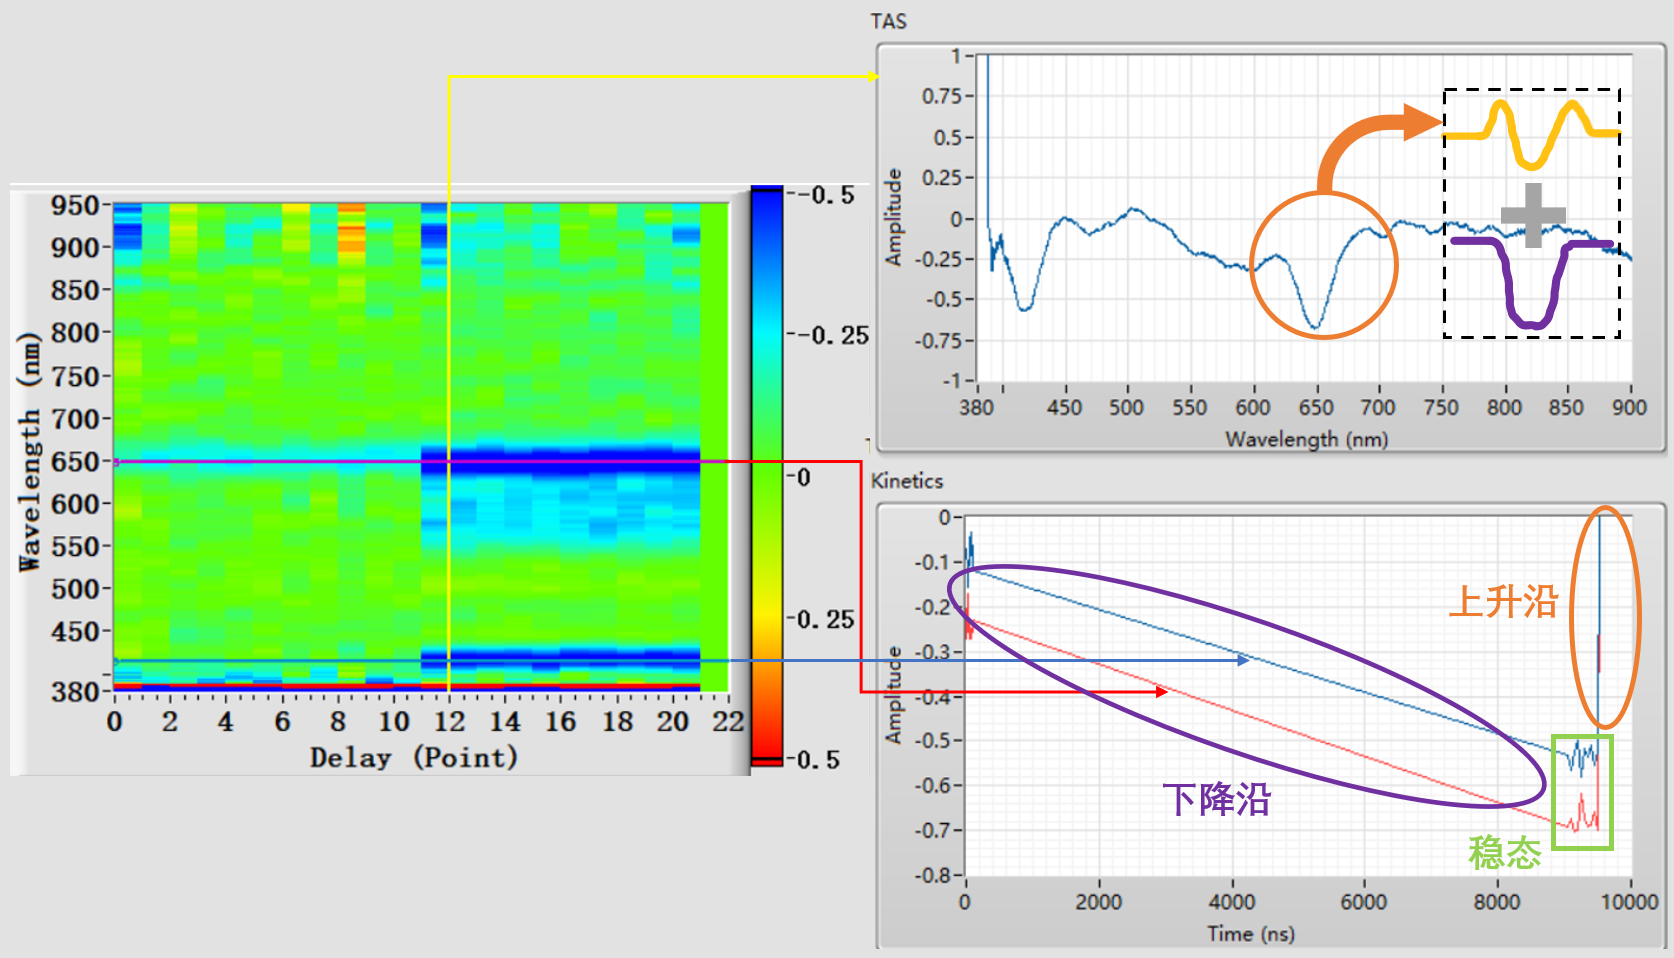
\includegraphics[width=\textwidth]{示例.png}
	\caption{EETA谱示例。}
	\label{fig:sl}
\end{figure}
\subsubsection{数据处理}
此前我们已经给出了电激发瞬态吸收光谱$\Delta A$的具体表达式(\ref{eq:3}),因此我们用以下形式拟合$\Delta A$进而将量子点漂白信号和斯塔克效应信号区分开:
\begin{equation}
	\Delta A=Bleaching+Stark=a\times A+\left(b\times \dfrac{\dif A}{\dif \lambda}+c\times\dfrac{\dif^2A}{\dif \lambda^2}\right).
	\label{eq:4}
\end{equation}
其中A是无电激发时样品的吸光度,我们知道基于朗伯比尔定律(Beer–Lambert Law),物质对光吸收的强弱与吸光物质的浓度和厚度有关,故探测光强度可以表示为$I=I_0\eu^{-2\sigma n_{QD}l_{QD}}$,故吸光度可以表示为:
\begin{equation}
	A=-\lg I/I_0=\dfrac{2\sigma n_{QD}l_{QD}}{2.303}.
	\label{eq:5}
\end{equation}
这里参数的定义同表达式(\ref{eq:3}),故不再赘述。对比表达式(\ref{eq:3})和表达式(\ref{eq:4})我们可以得到:
\begin{equation}
	a=-N_e.\quad b=(1-N_e)\left(E\dfrac{\partial \nu}{\partial E}+E^2\dfrac{\partial^2 \nu}{\partial E^2}\right).\quad c=(1-N_e)E^2\left(\dfrac{\partial \nu}{\partial E}\right)^2.
	\label{eq:6}
\end{equation}
进而,我们可以根据对比系数来获取QD-LED在电致发光中载流子动力学和电场信息。
\section{本章小结}
本章主要是围绕电激发瞬态吸收光谱技术展开,首先简单介绍了泵浦-探测技术,然后我们介绍了瞬态吸收光谱中主要的四个信号组成,接着我们介绍了电激发瞬态吸收光谱技术,说明其相对于传统光激发瞬态吸收光谱技术在QD-LED领域的优势并给出了电激发瞬态吸收光谱的表达形式,指出其主要是由Bleaching信号和Stark信号贡献。下面,我们给出了本文的一项工作,即搭建了一台可用于探测ZnO目标波段的紫外拓展的电激发瞬态吸收光谱仪,并指出了其中的一些细节部分,还简单展示了我们的LabVIEW操控系统。最后,我们介绍了处理数据的方法,顺带介绍了Bleaching信号和Stark信号在TAS中的影响。